\documentclass{ctexart}

\usepackage{graphicx}
\usepackage{amsmath}
\usepackage{tikz}
\usepackage{gnuplot-lua-tikz}
\usetikzlibrary{positioning, shapes.geometric}

\title{作业六: 介绍一元二次方程在实数域上的求解}

\author{作者姓名 罗俊勋 \\ 作者专业和学号 统计学 3210103619}

\begin{document}

\maketitle

\section{一元二次方程}
$ax^2+bx+c=0(a \neq 0)$


\section{一元二次方程求解的算法流程图}

\begin{tikzpicture}[node distance=10pt]
  \node[draw, rounded corners]                        (start) 
  {$ax^2+bx+c=0(a \neq 0)$};
  \node[draw, below=of start]                         (step 1)
  {$x^2+\frac{b}{a}x+(\frac{b}{2a})^2=-\frac{c}{a}+(\frac{b}{2a})^2(a \neq 0)$};
  \node[draw, below=of step 1]                        (step 2)
  {$(x+\frac{b}{2a})^2=-\frac{c}{a}+(\frac{b}{2a})^2(a \neq 0)$};
  \node[draw, diamond, aspect=3, below=of step 2]     (choice)
  {$\Delta=-\frac{c}{a}+(\frac{b}{2a})^2$};
  \node[draw, below=40pt of choice]  (step 3)
  {$x_1=\frac{-b+\sqrt{b^2-4ac}}{2a}\quad x_2=\frac{-b-\sqrt{b^2-4ac}}{2a}$};
  \node[draw, right=40pt of choice]  (step 4)
  {$x_1=x_2=\frac{-b}{2a}$};
  \node[draw, left=40pt of choice]  (step 5)
  {无实根};
  
  \draw[->] (start)  -- (step 1);
  \draw[->] (step 1) -- (step 2);
  \draw[->] (step 2) -- (choice);
  \draw[->] (choice) -- node[left]  {$\Delta>0$}
  (step 3);
  \draw[->] (choice) -- node[above] {$\Delta=0$}
  (step 4);
  \draw[->] (choice) -- node[above] {$\Delta<0$}
  (step 5);
\end{tikzpicture}

\section{一元二次方程解的三种情况的示意图}

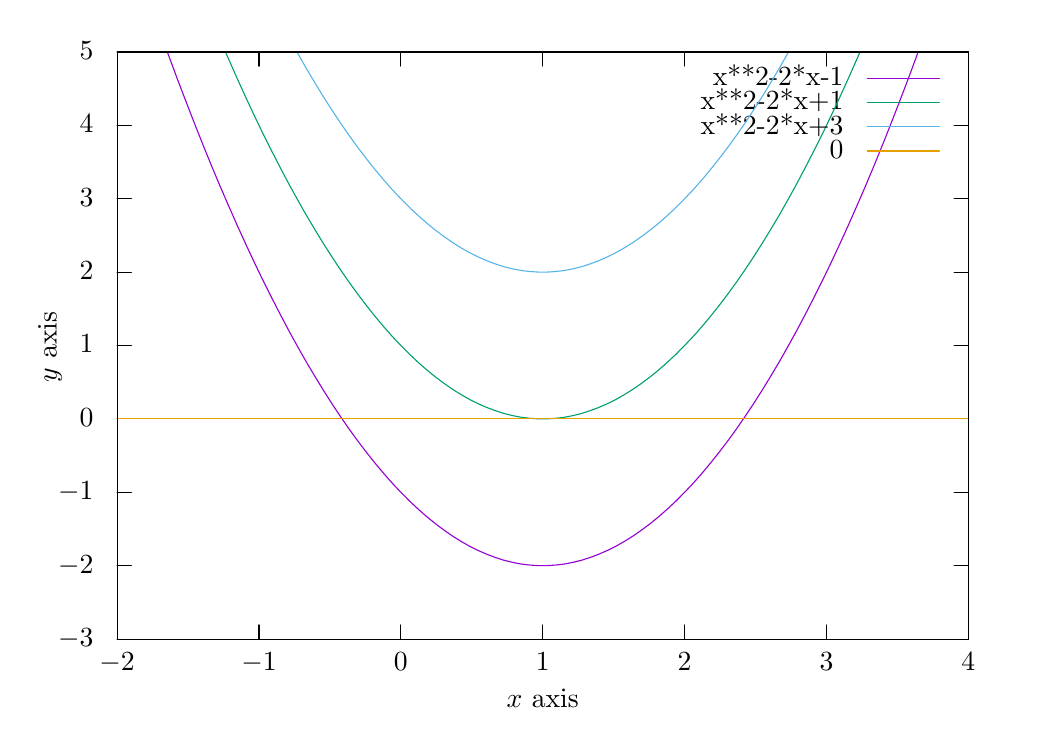
\begin{tikzpicture}[gnuplot]
%% generated with GNUPLOT 5.2p8 (Lua 5.3; terminal rev. Nov 2018, script rev. 108)
%% 2022年07月03日 星期日 23时00分12秒
\path (0.000,0.000) rectangle (12.500,8.750);
\gpcolor{color=gp lt color border}
\gpsetlinetype{gp lt border}
\gpsetdashtype{gp dt solid}
\gpsetlinewidth{1.00}
\draw[gp path] (1.136,0.985)--(1.316,0.985);
\draw[gp path] (11.947,0.985)--(11.767,0.985);
\node[gp node right] at (0.952,0.985) {$-3$};
\draw[gp path] (1.136,1.917)--(1.316,1.917);
\draw[gp path] (11.947,1.917)--(11.767,1.917);
\node[gp node right] at (0.952,1.917) {$-2$};
\draw[gp path] (1.136,2.849)--(1.316,2.849);
\draw[gp path] (11.947,2.849)--(11.767,2.849);
\node[gp node right] at (0.952,2.849) {$-1$};
\draw[gp path] (1.136,3.781)--(1.316,3.781);
\draw[gp path] (11.947,3.781)--(11.767,3.781);
\node[gp node right] at (0.952,3.781) {$0$};
\draw[gp path] (1.136,4.713)--(1.316,4.713);
\draw[gp path] (11.947,4.713)--(11.767,4.713);
\node[gp node right] at (0.952,4.713) {$1$};
\draw[gp path] (1.136,5.645)--(1.316,5.645);
\draw[gp path] (11.947,5.645)--(11.767,5.645);
\node[gp node right] at (0.952,5.645) {$2$};
\draw[gp path] (1.136,6.577)--(1.316,6.577);
\draw[gp path] (11.947,6.577)--(11.767,6.577);
\node[gp node right] at (0.952,6.577) {$3$};
\draw[gp path] (1.136,7.509)--(1.316,7.509);
\draw[gp path] (11.947,7.509)--(11.767,7.509);
\node[gp node right] at (0.952,7.509) {$4$};
\draw[gp path] (1.136,8.441)--(1.316,8.441);
\draw[gp path] (11.947,8.441)--(11.767,8.441);
\node[gp node right] at (0.952,8.441) {$5$};
\draw[gp path] (1.136,0.985)--(1.136,1.165);
\draw[gp path] (1.136,8.441)--(1.136,8.261);
\node[gp node center] at (1.136,0.677) {$-2$};
\draw[gp path] (2.938,0.985)--(2.938,1.165);
\draw[gp path] (2.938,8.441)--(2.938,8.261);
\node[gp node center] at (2.938,0.677) {$-1$};
\draw[gp path] (4.740,0.985)--(4.740,1.165);
\draw[gp path] (4.740,8.441)--(4.740,8.261);
\node[gp node center] at (4.740,0.677) {$0$};
\draw[gp path] (6.542,0.985)--(6.542,1.165);
\draw[gp path] (6.542,8.441)--(6.542,8.261);
\node[gp node center] at (6.542,0.677) {$1$};
\draw[gp path] (8.343,0.985)--(8.343,1.165);
\draw[gp path] (8.343,8.441)--(8.343,8.261);
\node[gp node center] at (8.343,0.677) {$2$};
\draw[gp path] (10.145,0.985)--(10.145,1.165);
\draw[gp path] (10.145,8.441)--(10.145,8.261);
\node[gp node center] at (10.145,0.677) {$3$};
\draw[gp path] (11.947,0.985)--(11.947,1.165);
\draw[gp path] (11.947,8.441)--(11.947,8.261);
\node[gp node center] at (11.947,0.677) {$4$};
\draw[gp path] (1.136,8.441)--(1.136,0.985)--(11.947,0.985)--(11.947,8.441)--cycle;
\node[gp node center,rotate=-270] at (0.292,4.713) {$y$ axis};
\node[gp node center] at (6.541,0.215) {$x$ axis};
\node[gp node right] at (10.479,8.107) {x**2-2*x-1};
\gpcolor{rgb color={0.580,0.000,0.827}}
\draw[gp path] (10.663,8.107)--(11.579,8.107);
\draw[gp path] (1.774,8.441)--(1.791,8.395)--(1.900,8.100)--(2.010,7.813)--(2.119,7.532)%
  --(2.228,7.258)--(2.337,6.991)--(2.446,6.731)--(2.556,6.478)--(2.665,6.231)--(2.774,5.992)%
  --(2.883,5.759)--(2.992,5.533)--(3.102,5.314)--(3.211,5.102)--(3.320,4.896)--(3.429,4.698)%
  --(3.538,4.506)--(3.648,4.321)--(3.757,4.143)--(3.866,3.972)--(3.975,3.808)--(4.084,3.650)%
  --(4.194,3.499)--(4.303,3.356)--(4.412,3.219)--(4.521,3.089)--(4.630,2.965)--(4.740,2.849)%
  --(4.849,2.739)--(4.958,2.637)--(5.067,2.541)--(5.176,2.452)--(5.286,2.370)--(5.395,2.294)%
  --(5.504,2.226)--(5.613,2.164)--(5.722,2.110)--(5.832,2.062)--(5.941,2.021)--(6.050,1.986)%
  --(6.159,1.959)--(6.268,1.938)--(6.378,1.925)--(6.487,1.918)--(6.596,1.918)--(6.705,1.925)%
  --(6.815,1.938)--(6.924,1.959)--(7.033,1.986)--(7.142,2.021)--(7.251,2.062)--(7.361,2.110)%
  --(7.470,2.164)--(7.579,2.226)--(7.688,2.294)--(7.797,2.370)--(7.907,2.452)--(8.016,2.541)%
  --(8.125,2.637)--(8.234,2.739)--(8.343,2.849)--(8.453,2.965)--(8.562,3.089)--(8.671,3.219)%
  --(8.780,3.356)--(8.889,3.499)--(8.999,3.650)--(9.108,3.808)--(9.217,3.972)--(9.326,4.143)%
  --(9.435,4.321)--(9.545,4.506)--(9.654,4.698)--(9.763,4.896)--(9.872,5.102)--(9.981,5.314)%
  --(10.091,5.533)--(10.200,5.759)--(10.309,5.992)--(10.418,6.231)--(10.527,6.478)--(10.637,6.731)%
  --(10.746,6.991)--(10.855,7.258)--(10.964,7.532)--(11.073,7.813)--(11.183,8.100)--(11.292,8.395)%
  --(11.308,8.441);
\gpcolor{color=gp lt color border}
\node[gp node right] at (10.479,7.799) {x**2-2*x+1};
\gpcolor{rgb color={0.000,0.620,0.451}}
\draw[gp path] (10.663,7.799)--(11.579,7.799);
\draw[gp path] (2.512,8.441)--(2.556,8.342)--(2.665,8.095)--(2.774,7.856)--(2.883,7.623)%
  --(2.992,7.397)--(3.102,7.178)--(3.211,6.966)--(3.320,6.760)--(3.429,6.562)--(3.538,6.370)%
  --(3.648,6.185)--(3.757,6.007)--(3.866,5.836)--(3.975,5.672)--(4.084,5.514)--(4.194,5.363)%
  --(4.303,5.220)--(4.412,5.083)--(4.521,4.953)--(4.630,4.829)--(4.740,4.713)--(4.849,4.603)%
  --(4.958,4.501)--(5.067,4.405)--(5.176,4.316)--(5.286,4.234)--(5.395,4.158)--(5.504,4.090)%
  --(5.613,4.028)--(5.722,3.974)--(5.832,3.926)--(5.941,3.885)--(6.050,3.850)--(6.159,3.823)%
  --(6.268,3.802)--(6.378,3.789)--(6.487,3.782)--(6.596,3.782)--(6.705,3.789)--(6.815,3.802)%
  --(6.924,3.823)--(7.033,3.850)--(7.142,3.885)--(7.251,3.926)--(7.361,3.974)--(7.470,4.028)%
  --(7.579,4.090)--(7.688,4.158)--(7.797,4.234)--(7.907,4.316)--(8.016,4.405)--(8.125,4.501)%
  --(8.234,4.603)--(8.343,4.713)--(8.453,4.829)--(8.562,4.953)--(8.671,5.083)--(8.780,5.220)%
  --(8.889,5.363)--(8.999,5.514)--(9.108,5.672)--(9.217,5.836)--(9.326,6.007)--(9.435,6.185)%
  --(9.545,6.370)--(9.654,6.562)--(9.763,6.760)--(9.872,6.966)--(9.981,7.178)--(10.091,7.397)%
  --(10.200,7.623)--(10.309,7.856)--(10.418,8.095)--(10.527,8.342)--(10.570,8.441);
\gpcolor{color=gp lt color border}
\node[gp node right] at (10.479,7.491) {x**2-2*x+3};
\gpcolor{rgb color={0.337,0.706,0.914}}
\draw[gp path] (10.663,7.491)--(11.579,7.491);
\draw[gp path] (3.420,8.441)--(3.429,8.426)--(3.538,8.234)--(3.648,8.049)--(3.757,7.871)%
  --(3.866,7.700)--(3.975,7.536)--(4.084,7.378)--(4.194,7.227)--(4.303,7.084)--(4.412,6.947)%
  --(4.521,6.817)--(4.630,6.693)--(4.740,6.577)--(4.849,6.467)--(4.958,6.365)--(5.067,6.269)%
  --(5.176,6.180)--(5.286,6.098)--(5.395,6.022)--(5.504,5.954)--(5.613,5.892)--(5.722,5.838)%
  --(5.832,5.790)--(5.941,5.749)--(6.050,5.714)--(6.159,5.687)--(6.268,5.666)--(6.378,5.653)%
  --(6.487,5.646)--(6.596,5.646)--(6.705,5.653)--(6.815,5.666)--(6.924,5.687)--(7.033,5.714)%
  --(7.142,5.749)--(7.251,5.790)--(7.361,5.838)--(7.470,5.892)--(7.579,5.954)--(7.688,6.022)%
  --(7.797,6.098)--(7.907,6.180)--(8.016,6.269)--(8.125,6.365)--(8.234,6.467)--(8.343,6.577)%
  --(8.453,6.693)--(8.562,6.817)--(8.671,6.947)--(8.780,7.084)--(8.889,7.227)--(8.999,7.378)%
  --(9.108,7.536)--(9.217,7.700)--(9.326,7.871)--(9.435,8.049)--(9.545,8.234)--(9.654,8.426)%
  --(9.662,8.441);
\gpcolor{color=gp lt color border}
\node[gp node right] at (10.479,7.183) {0};
\gpcolor{rgb color={0.902,0.624,0.000}}
\draw[gp path] (10.663,7.183)--(11.579,7.183);
\draw[gp path] (1.136,3.781)--(1.245,3.781)--(1.354,3.781)--(1.464,3.781)--(1.573,3.781)%
  --(1.682,3.781)--(1.791,3.781)--(1.900,3.781)--(2.010,3.781)--(2.119,3.781)--(2.228,3.781)%
  --(2.337,3.781)--(2.446,3.781)--(2.556,3.781)--(2.665,3.781)--(2.774,3.781)--(2.883,3.781)%
  --(2.992,3.781)--(3.102,3.781)--(3.211,3.781)--(3.320,3.781)--(3.429,3.781)--(3.538,3.781)%
  --(3.648,3.781)--(3.757,3.781)--(3.866,3.781)--(3.975,3.781)--(4.084,3.781)--(4.194,3.781)%
  --(4.303,3.781)--(4.412,3.781)--(4.521,3.781)--(4.630,3.781)--(4.740,3.781)--(4.849,3.781)%
  --(4.958,3.781)--(5.067,3.781)--(5.176,3.781)--(5.286,3.781)--(5.395,3.781)--(5.504,3.781)%
  --(5.613,3.781)--(5.722,3.781)--(5.832,3.781)--(5.941,3.781)--(6.050,3.781)--(6.159,3.781)%
  --(6.268,3.781)--(6.378,3.781)--(6.487,3.781)--(6.596,3.781)--(6.705,3.781)--(6.815,3.781)%
  --(6.924,3.781)--(7.033,3.781)--(7.142,3.781)--(7.251,3.781)--(7.361,3.781)--(7.470,3.781)%
  --(7.579,3.781)--(7.688,3.781)--(7.797,3.781)--(7.907,3.781)--(8.016,3.781)--(8.125,3.781)%
  --(8.234,3.781)--(8.343,3.781)--(8.453,3.781)--(8.562,3.781)--(8.671,3.781)--(8.780,3.781)%
  --(8.889,3.781)--(8.999,3.781)--(9.108,3.781)--(9.217,3.781)--(9.326,3.781)--(9.435,3.781)%
  --(9.545,3.781)--(9.654,3.781)--(9.763,3.781)--(9.872,3.781)--(9.981,3.781)--(10.091,3.781)%
  --(10.200,3.781)--(10.309,3.781)--(10.418,3.781)--(10.527,3.781)--(10.637,3.781)--(10.746,3.781)%
  --(10.855,3.781)--(10.964,3.781)--(11.073,3.781)--(11.183,3.781)--(11.292,3.781)--(11.401,3.781)%
  --(11.510,3.781)--(11.619,3.781)--(11.729,3.781)--(11.838,3.781)--(11.947,3.781);
\gpcolor{color=gp lt color border}
\draw[gp path] (1.136,8.441)--(1.136,0.985)--(11.947,0.985)--(11.947,8.441)--cycle;
%% coordinates of the plot area
\gpdefrectangularnode{gp plot 1}{\pgfpoint{1.136cm}{0.985cm}}{\pgfpoint{11.947cm}{8.441cm}}
\end{tikzpicture}
%% gnuplot variables


\end{document}
